% !TEX root =  main.tex
\section{Introduction}
\subsection{Motivation}

Building systems that can understand and reason with information present in texts is a central pursuit in the AI vision. Extracting and understanding information in texts itself requires background knowledge. It is no surprise that documents written for human consumption assume background knowledge and an inference capability that reads between lines. For example, consider the following news snippet:

\begin{verbatim}
        Somalia's al-Shabab militant group has confirmed the death 
        of its leader in a U.S. airstrike and named his successor. 
        The al-Qaida linked militants announced the selection of 
        Abu Ubeid Ahmed Omar to replace Abdi Godane. 
\end{verbatim}

Reading these two sentences, we can easily conclude that {\em Abdi Godane} was the leader of {\em al-Shabab}, which is a {\em terrorist group} and {\em Abu Ubeid Ahmed Omar} is the successor of {\em Abdi Godane}, and {\em Abdi Godane} was killed by a {\em U.S.} airstrike. None of this information is explicitly mentioned in the sentences but can be {\em easily} inferred by humans. However, this inference is not so {\em easy} for extraction systems. 

Most information extraction systems target binary relations hat were explicitly mentioned in texts and cannot account for the implicit or inferred relations easily. Even within the explicitly expressed relations, many closed-domain IE systems can only extract a small set of manually pre-specified relations limiting their use to a small number of domains. On the other hand, Open IE systems extract every possible relation explicitly stated in text and do not have any notion of salience or importance to the main events in the discourse. Furthermore, binary relations do not capture the complexity of events that have multiple actors who perform specific roles within the event. 

To effectively address these issues, extraction systems need background knowledge that provide models or expectations for the information they need to extract. For example models of salient aspects of certain types of entities (e.g., actors {\em act in} movies, actors {\em win} awards) can help extract and organize information about people. Similarly, rich descriptions of events or scenarios, processes and their interactions can help in extracting and understanding information about events from texts. Scalable methods for acquiring such background knowledge is essential for building broad coverage extractors.

Template-driven extraction aims to address these issues by pre-specifying an extraction template for each event type (e.g., arrest, arson, bombing). The template describes an event type in terms of the actors and the roles they play within the event. Figure~\ref{fig:arrest} shows an example arrest template (or schema).  
\begin{wrapfigure}{lh}{0.4\textwidth}
	\vspace{-2ex}
	\begin{center}
	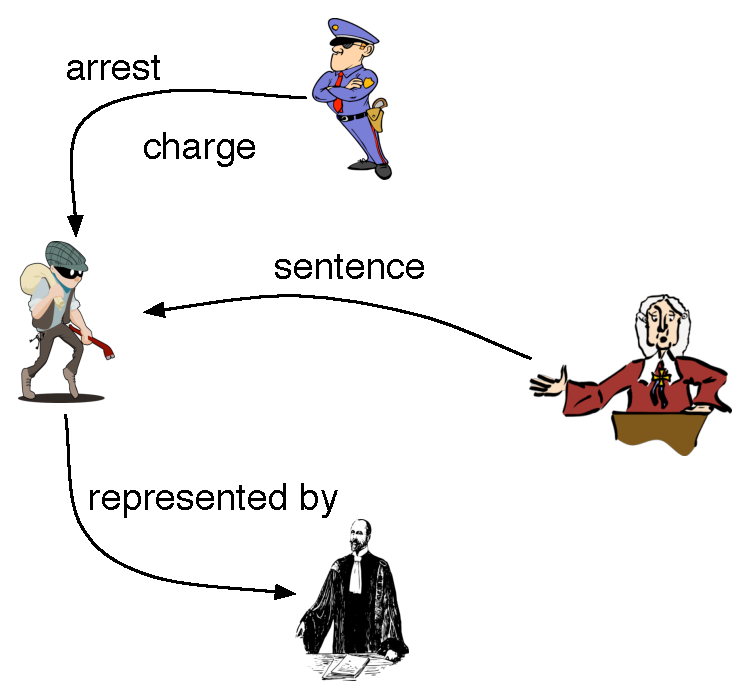
\includegraphics[width=2.5in,height=2in]{figures/arrest-scenario} 	
	\caption{\label{fig:arrest} {Arrest schema: A model for an arrest scenario with the key actors and their roles.}}
	\end{center}
\end{wrapfigure}
The key actors are an arresting agent who arrests and charges a suspect, a lawyer who represents the suspect and a judge who rules on the case. 

However, templates are fundamentally limited by the cost of manual authoring. Chambers and Jurafsky (2009) developed an automatic method for generating event schemas that scaled to arbitrary domains but used a simple representation that resulted in schemas that were mostly incoherent because they mixed distinct events (e.g., fire spreading vs. disease spreading). 

In this work, we target extraction of rich schemas that describe events using a range of information as shown in the table below.

\begin{table}[htdp]
\caption{default}
\begin{center}
\begin{tabular}{|p{4cm}|p{12cm}|}
\hline
Entities & Extractors\\
& Researcher, Organization, Subject, Problem, Conclusion, Publication, Date, Location \\
\hline
Sub-events &  \\
& R: Researcher study Problem (X)\\
& R find found/discovered/uncovered/stumbled/ Conclusion (Y) \\
& R published Results/Conclusions in [Journal/Book/Conference] \\
& R supports/refutes \\
& \\
\hline
Background-relations & \\
& R: Researcher, employed by, O:[Organization] \\
& study: Research, funded by, O:[Organization] \\
\hline
Entity Extractors & \\
& X:[Person] studies Y: [Problem] $\rightarrow$ X: [Researcher] \\
& X is studied by Y: [Person] $\rightarrow$ X: [Subject]\\
& X: [Researcher] concludes Y $\rightarrow$ Y: [Conclusion]\\
\hline
Relation Extractors & \\
	& study -- studied, investigated, explored, asked\\
	& find -- discovered, uncovered, stumbled \\			
\hline
Dependencies (Rel-grams) & \\
& R found Y, Conclusion(Y) $\rightarrow$ R publishes Y \\
& R found Y, Conclusion(Y) $\rightarrow$ R studied X \\	
\hline
Related Scripts & \\
& investigate, publish \\
\hline
\end{tabular}
\end{center}
\label{default}
\end{table}%


In preliminary work, we generated {\em coherent} event schemas for arbitrary domains. It leveraged the scalability of Open Information Extraction to produce a representation that included more context and used a simple generalization of the arguments to address sparsity. 

%These open-domain event schemas are but a starting point for aggregating and organizing background knowledge about events that can be leveraged during extraction. The main goal of this project is to build open-domain script like knowledge about events. 

Script-like knowledge serve as general purpose description of events or scenarios. In addition to the key actors, their actions, we will build scripts that include causal, temporal and dependency relationships between the different actions. During extraction this richer representation will enable us to infer more than what is explicitly mentioned in the text. 

Schemas provide a high precision model of scenarios which can be expanded to associated extractors -- i.e., patterns that can be used to extract from new texts. Resolving entity and event co-references. Third, scripts must include causal and temporal ordering of the actions in a scenario. 

\subsection{Research Challenges}



\subsection{Contributions}
